\documentclass[12pt]{amsart}

\usepackage{fullpage, amsmath, amsthm, amssymb, verbatim, graphicx}

\newcommand{\RR}{\mathbb{R}}
\newcommand{\ZZ}{\mathbb{Z}}
\DeclareMathOperator{\rref}{rref}
\DeclareMathOperator{\nullity}{nullity}
\DeclareMathOperator{\Span}{span}
\DeclareMathOperator{\rank}{rank}

\newtheorem{theorem}{Theorem}[section]
\newtheorem{thdf}{Theorem-Definition}[section]
\newtheorem{corollary}[theorem]{Corollary} \newtheorem{lemma}[theorem]{Lemma}
\theoremstyle{definition} \newtheorem{definition}[theorem]{Definition}
\newtheorem{provdef}[theorem]{Provisional definition}
\newtheorem{definitions}[theorem]{Definitions}
\newtheorem{remark}[theorem]{Remark} \newtheorem{remarks}[theorem]{Remarks}
\newtheorem{example}[theorem]{Example}
\newtheorem{exdef}[theorem]{Example-Definition}
\newtheorem{exercise}[theorem]{Exercise}

\newcommand{\ba}{\mathbf{a}}
\newcommand{\bb}{\mathbf{b}}
\newcommand{\bc}{\mathbf{c}}
\newcommand{\bd}{\mathbf{d}}
\newcommand{\be}{\mathbf{e}}
\newcommand{\bi}{\mathbf{i}}
\newcommand{\bu}{\mathbf{u}}
\newcommand{\bv}{\mathbf{v}}
\newcommand{\bw}{\mathbf{w}}
\newcommand{\bx}{\mathbf{x}}
\newcommand{\by}{\mathbf{y}}
\newcommand{\bz}{\mathbf{z}}
\newcommand{\bzero}{\mathbf{0}}

\newcommand{\bas}{\ba_1,\ldots,\ba_n}
\newcommand{\mat}[1]{\begin{bmatrix}#1\end{bmatrix}}
\newcommand{\Rmn}{\RR^{m\times n}} \newcommand{\Rmm}{\RR^{m\times m}}
\newcommand{\Rnn}{\RR^{n\times n}}
\newcommand{\spn}[1]{\Span\left(#1\right)}

\newcommand{\setstuff}{\setlength{\parskip}{0.5em}\setlength{\parindent}{0em}\setlength{\itemsep}{0.5em}}

\begin{document}
\setstuff


\section{The equation $A\bx=\bb$}

Let $A\in\RR^{m\times n}$.
The nature of the solution set of the equation $A\bx=\bb$, for $\bb\in\RR^m$, is governed by two sets:

\begin{definition}\label{df:col_space}\hfill
  \begin{enumerate}\setstuff
    \item The set
    \[ N(A) = \{\bx\in\RR^n : A\bx=\bzero\} \]
      is called the \emph{nullspace of $A$}. It's the solution set of the homogeneous equation $A\bx=\bzero$.
   \item The set
     \[ C(A) := \{\bb\in\RR^m :	\bb=A\bx,\text{ for some }\bx\in\RR^n\} \]
    is called the \emph{column space of $A$}. It's the set of vectors $\bb\in\RR^m$ for which the equation $A\bx=\bb$ has a solution.
  \end{enumerate}
\end{definition}

To determine $N(A)$ is to solve the equation $A\bx=\bzero$.
\begin{example}\label{eg:nullspace}
  Let
  \[
    A = \mat{1&4&7\\2&5&8\\3&6&9}.
  \]
  The nullspace of $A$ is the solution set of
  \[
    \mat{1&4&7\\2&5&8\\3&6&9}\mat{x_1\\x_2\\x_3}=\mat{0\\0\\0}:
  \]
  \[
    N(A) =\left\{t\mat{1\\-2\\1} : t\in\RR\right\}.
  \]
\end{example}

\begin{example}\label{eg:nullspace}
  Let
  \[
    A = \mat{1&2&3\\4&5&6\\7&8&9}.
  \]
  Setting
  \[
    \bb=\mat{b_1\\b_2\\b_3}\in\RR^3,
  \]
  and going through the motions of solving the system
  \begin{equation*}
    \mat{1&2&3\\4&5&6\\7&8&9}\mat{x_1\\x_2\\x_3}=\mat{b_1\\b_2\\b_3},
    \tag{\maltese}
  \end{equation*}
  we identify a condition under which $\bb$ belongs to $C(A)$.

  Application of two elementary row operations (which ones?) transforms 
  \[
    \mat{A&\bb}=\mat{1&2&3&b_1\\4&5&6&b_2\\7&8&9&b_3},
  \]
  the augmented matrix of (\maltese), into
  \[
    \mat{1&2&3&b_1\\0&-3&-6&b_2-4b_1\\0&0&0&b_1-2b_2+b_3},
  \]
  It follows that $A\bx=\bb$ has a solution if and only if $b_1-2b_2+b_3 = 0$. Thus,
  \[
    C(A) = \left\{\mat{b_1\\b_2\\b_3} : b_1-2b_2+b_3=0\right\}.
  \]
  Note that this description makes it easy to test a vector $\bb$ for membership in $C(A)$ --- simply check whether $b_1-2b_2+b_3$ is $0$ or not.

  Finally, notice that
  \begin{align*}
    C(A) %&= \left\{\mat{b_1\\b_2\\b_3} : b_1-2b_2+b_3=0\right\}\\
         &= \left\{\mat{b_1\\b_2\\b_3} :
         \mat{1&-2&1}\mat{b_1\\b_2\\b_3} = 0 \right\}\\
               &= N\left(\mat{1&-2&1}\right).
  \end{align*}
  The column space of one matrix can be the nullspace of another! 
\end{example}

\begin{exercise}\label{ex:invertible_nullsapce_col_space}
  Let $A\in\RR^{m\times m}$ be an invertible matrix. Prove that $N(A)=\{\bzero\}$ and that $C(A)=\RR^m$.
%  The identity $N(A)=\{\bzero\}$ follows from the fact that $A\bx=\bzero$ if and only if $\bx=A^{-1}\bzero=\bzero$.
%  Let $\bv\in\RR^m$. Then $A\bx=\bb$ has solution $\bx=A^{-1}\bb$, putting $\bb$ in $C(A)$. Since $\bv\in\RR^m$ was arbitrary, $C(A)=\RR^m$.
\end{exercise}

The set $C(A)$ governs the solubility of $A\bx=\bb$, while $N(A)$ determines the size of the corresponding set. More precisely:

\begin{theorem}\label{th:particular_plus_general}
  Let $\bb\in C(A)$, so that $A\bx=\bb$ has at least one solution, $\bx_0$, say. Then
      \begin{equation*}
        \{\bx : A\bx=\bb\} = \{\bx_0 + \by : \by\in N(A)\}.
  \end{equation*}
\end{theorem}

\begin{proof}
Let $\bb\in C(A)$.
Let $\bx\in \{\bx : A\bx=\bb\}$.
Then
  \[
    A(\bx-\bx_0) = A\bx - A\bx_0 = \bb - \bb = \bzero.
  \]
  Thus, $\by := \bx-\bx_0\in N(A)$ and $\bx = \bx_0 + \by$.
  Therefore, $\bx\in \{\bx_0 + \by : \by\in N(A)\}$.
  Since $\bx\in \{\bx : A\bx=\bb\}$ was arbitrary,
  \[
    \{\bx : A\bx=\bb\}\subseteq\{\bx_0 + \by : \by\in N(A)\}.
  \]

  Conversely, suppose $\bx\in \{\bx_0 + \by : \by\in N(A)\}$, i.e., $\bx = \bx_0 + \by$, for some $\by\in N(A)$.
  Now $A\bx_0=\bzero$ by hypothesis and $A\by=\bzero$ by definition of $N(A)$.
  Therefore,
  \[
    A\bx = A(\bx_0 + y) = A\bx_0 + A\by = \bzero + \bzero = \bzero.
  \]
  Thus, $\bx\in N(A)$.
  Since $\bx\in \{\bx_0 + \by : \by\in N(A)\}$ was arbitrary,
  \[
    \{\bx_0 + \by : \by\in N(A)\}\subseteq \{\bx : A\bx=\bb\}.
  \]
  Having proved the reverse containment above, equality holds. 
\end{proof}

\begin{example}
  Let
  \[
    A = \mat{1&4&7\\2&5&8\\3&6&9}.
  \]
  Since
  \[
    \mat{1&4&7\\2&5&8\\3&6&9}\mat{1\\1\\0} = \mat{5\\7\\9} =: \bb
  \]
  and, by Example~\ref{eg:nullspace}, 
  \[
    N(A) =\left\{t\mat{1\\-2\\1} : t\in\RR\right\},
  \]
  Theorem~\ref{th:particular_plus_general} implies that
  \[
    \left\{\bx : A\bx=\bb\right\} =
    \left\{\mat{1\\1\\0} + t\mat{1\\-2\\1}: t\in\RR\right\}.
  \]
\end{example}

\section{Subspaces}

\begin{definition}\label{df:subspace}
  A subset $U$ of $\RR^m$ is a \emph{subspace of $\RR^m$} if:
  \begin{enumerate}
    \item The zero vector of $\RR^m$ belongs to $U$:
      \[
        \bzero\in U.
      \]
    \item $U$ is \emph{closed under addition}:
      \begin{center}
        If $\bu_1\in U$ and $\bu_2\in U$ then $\bu_1+\bu_2\in U$.
      \end{center}
    \item $U$ is \emph{closed under scalar multiplication}:
      \begin{center}
        If $\bu\in U$ and $s\in \RR$ then $s\bu\in U$.
      \end{center}
  \end{enumerate}
\end{definition}

\begin{remarks}\hfill
  \begin{itemize}
\item When attempting to prove that a subset $U$ of $\RR^m$ satisfies property (2), you need to show that $\bu_1+\bu_2\in U$ for \emph{any} pair of elements $\bu_1, \bu_2$ of $U$.
  Similarly, to prove that a subset $U$ of $\RR^m$ satisfies property (3), you need to show that $s\bu\in U$ for \emph{any} element $\bu_1$ of $U$ and \emph{any} real number $s$.

\item To show that a given subset $U$ of $\RR^m$ is \emph{not} a subspace of $\RR^m$, you need only show that \emph{one of} (1), (2), and (3) fail.
  To show that (2) fails, you need only produce \emph{one} pair $\bu_1, bu_2$ of elements of $U$ such that $\bu_1+\bu_2\notin U$.
  Similarly, to prove that (3) fails, you need only produce \emph{one} element $\bu$ of $U$ and \emph{one} real number $s$ such that $s\bu \notin U$.
  \end{itemize}
\end{remarks}

\begin{example}\label{eg:nullspace_in_disguise}
  Let
  \[
    U = \left\{\mat{x\\y}\in\RR^2 : x+y=0\right\}.
  \]
  Then $U$ is a subspace of $\RR^2$. We prove this by verifying that $U$ satisfies properties (1), (2), and (3) of Definition~\ref{df:subspace}:
  \begin{enumerate}
    \item Since $0+0=0$,
    \[
      \bzero=\mat{0\\0}\in U,
    \]
    by defintion of $U$.

  \item Let
    \[
      \mat{x_1\\y_2},\mat{x_2\\y_2}\in U.
    \]
    Then, by definition of $U$,
    \[
      x_1+y_1=0\quad\text{and}\quad x_2+y_2=0.
    \]
    Therefore,
    \[
      (x_1+x_2) + (y_1+y_2) = (x_1+y_1) + (x_2+y_2)=0.
    \]
    Thus,
    \[
      \mat{x_1\\y_1} + \mat{x_2\\y_2} =
      \mat{x_1+x_2\\y_1+y_2}\in U,
    \]
    by definition of $U$.
    
  \item Let
    \[
      \mat{x\\y}\in U,\quad s\in \RR.
    \]
    Then, by defintion of $U$, we have 
    \[
      x+y=0.
    \]
    Therefore,
    \[
      sx+xy = s(x+y) =s(0) = 0.
    \]
    Thus,
    \[
      s\mat{x\\y} = \mat{sx\\sy}\in U.
    \]
 \end{enumerate}
\end{example}

\begin{example}
  Let
  \[
    U = \left\{\mat{x\\y}\in\RR^2 : x^2 + y^2 = 1\right\}.
  \]
  Then $U$ is not a subspace of $\RR^2$ as $\bzero\notin U$:
  \[
    0^2 + 0^2 = 0 \neq 1.
  \]
\end{example}

\begin{example}
  Let
  \[
    U = \left\{\mat{x\\y}\in\RR^2 : x^2 = y^2\right\}.
  \]
  Then $U$ is not a subspace of $\RR^2$ since it fails property (2) of Definition~\ref{df:subspace}:
  \begin{center}
    $\mat{1\\1}, \mat{1\\-1}\in U$,
    but $\mat{1\\0}=\mat{1\\1} + \mat{1\\-1}\notin U$.
  \end{center}
\end{example}

\begin{example}
  Let $\ZZ$, the set of integers, viewed as a subset of in $\RR=\RR^1$.
  Then $\ZZ$ is not a subspace of $\RR^1$ as $1\in \ZZ$ but
  \[
    \tfrac12\cdot 1 = \tfrac12\notin \ZZ.
  \]
\end{example}

\begin{theorem}\label{th:nullspace_is_subspace}
  Let $A\in\RR^{m\times n}$. Then $N(A)$ is a subspace of $\RR^n$.
\end{theorem}

\begin{proof} We prove properties (1), (2), and (3) of Definition~\ref{df:subspace}.
  \begin{enumerate}
    \item Since $A\bzero=\bzero$ we have $\bzero\in N(A)$ by defintion of $N(A)$.
    \item Let $\bx_1$ and $\bx_2$ be arbitrary elements of $N(A)$. Then, by definition of $N(A)$,
      \[
        A\bx_1=\bzero\quad\text{and}\quad A\bx_2=\bzero.
      \]
      Therefore,
      \[
        A(\bx_1+\bx_2) = A\bx_1 + A\bx_2 = \bzero + \bzero = \bzero.
      \]
      Thus, $\bx_1+\bx_2\in N(A)$, by definition of $N(A)$.
    \item Let $\bx$ be an arbitrary element of $N(A)$ and let $s$ be an y real number.
      As $\bx\in N(A)$, we have $A\bx=\bzero$, by defintion of $N(A)$.
      Therefore,
      \[
        A(s\bx) = s(A\bx) = s\bzero = \bzero.
      \]
      Thus, $s\bx\in N(A)$, by definition of $N(A)$.\qedhere
  \end{enumerate}
\end{proof}

\begin{example}
  We give a shorter proof that the set $U$ of Example~\ref{eg:nullspace_in_disguise} is a subspace of $\RR^2$.
  By the identity
  \[
    \mat{1&1}\mat{x\\y} = \mat{x+y},
  \]
  and the defintion of $N\left(\mat{1&1}\right)$, we have
  \begin{align*}
    U &= \left\{\mat{x\\y} : x + y = 0\right\}\\
      &= \left\{\mat{x\\y} : \mat{1& 1}\mat{x\\y} =
        \mat{0}\right\}\\
      &= N\left(\mat{1&1}\right).
  \end{align*}
  Therefore, by Theorem~\ref{th:nullspace_is_subspace}, $U$ is a subspace of $\RR^2$.

\begin{example}
  Let
  \[
    U = \left\{\mat{x\\y\\z} : \text{$x + 2y = 3z$ and
    $4z - 2x = y$}\right\}.
  \]
  We have:
  \begin{align*}
    &x+2y=3z& &\Longleftrightarrow& \mat{1&2&-3}\mat{x\\y\\z}&=\mat{0}\\
    \text{and}\qquad& 4z-2x=y& &\Longleftrightarrow& 
    \mat{-2&-1&4}\mat{x\\y\\z}&=\mat{0}.
  \end{align*}
  If follows that
  \[
    \mat{x\\y\\z}\in U\Longleftrightarrow
    \mat{1&2&-3\\-2&-1&4}\mat{x\\y\\z}=\mat{0\\0}.
  \]
  Therefore,
  \[
    U = N\left(\mat{1&2&-3\\-2&-1&4}\right),
  \]
  by definition of nullspace.
  Thus, by Theorem~\ref{th:nullspace_is_subspace}, $U$ is a subspace of $\RR^3$.

\end{example}

\end{example}

\begin{theorem}\label{th:col_space_is_subspace}
  Let $A\in\RR^{m\times n}$. Then $C(A)$ is a subspace of $\RR^m$.
\end{theorem}

\begin{proof} We prove properties (1), (2), and (3) of Definition~\ref{df:subspace}.
  \begin{enumerate}
    \item Since $\bzero = A\bzero$ we have $\bzero\in C(A)$, by defintion of $C(A)$.
    \item Let $\bb_1$ and $\bb_2$ be arbitrary elements of $C(A)$. Then, by definition of $C(A)$, there are elements $\bx_1$ and $\bx_2$ of $\RR^n$ such that
      \[
        A\bx_1=\bb_1\quad\text{and}\quad A\bx_2=\bb_2.
      \]
      Therefore,
      \[
        A(\bx_1+\bx_2) = A\bx_1 + A\bx_2 = \bb_1 + \bb_2.
      \]
      Thus, $\bb_1+\bb_2\in C(A)$, by definition of $C(A)$.
    \item Let $\bb$ be an arbitrary element of $C(A)$ and let $s$ be an y real number.
      As $\bb\in C(A)$, there is a vector $\bx$ in $\RR^n$ such that $A\bx=\bb$, by defintion of $C(A)$.
      Therefore,
      \[
        A(s\bx) = s(A\bx) = s\bb.
      \]
      Thus, $s\bb\in C(A)$, by definition of $C(A)$.\qedhere
  \end{enumerate}
\end{proof}

\begin{example}
  Let
  \[
    U =\left\{\mat{2x+3y\\y-x\\y}\in\RR^3 : s, t\in\RR,\right\}.
  \]
  By the identity
  \[
    \mat{2x+3y\\y-x\\y} = \mat{2&3\\-1&1\\0&1}\mat{x\\y},
  \]
  and the defintion of column space, we have
  \[
    U = C\left(\mat{2&3\\-1&1\\0&1}\right).
  \]
  Therefore, by Theorem~\ref{th:col_space_is_subspace}, $U$ is a subspace of $\RR^3$.
\end{example}

\begin{example}\label{eg:null_to_column}
  Let
  \[
    A = \mat{1&2&3&4\\5&6&7&8\\9&12&11&12}.
  \]
  The general solution of $A\bx=\bzero$ is
  \[
    \mat{w\\x\\y\\z} = s\mat{1\\-2\\1\\0} + t\mat{2\\-3\\0\\1}.
  \]
  By definition of nullspace,
  \[
    N(A) = \left\{s\mat{1\\-2\\1\\0} + t\mat{2\\-3\\0\\1} : s,t\in\RR\right\}
  \]
  By the identity
  \[
    s\mat{1\\-2\\1\\0} + t\mat{2\\-3\\0\\1} =
    \mat{1&2\\-2&-3\\1&0\\0&1}\mat{s\\t}
  \]
  and the definitions of nullspace and column space, it follows that
  \[
    N(A) = C\left(\mat{1&2\\-2&-3\\1&0\\0&1}\right).
  \]
\end{example}

\begin{remarks}\hfill
  \begin{itemize}
    \item Example~\ref{eg:null_to_column} illustrates that ``solving the system'' $A\bx=\bb$, in the sense of MATH 211, amounts to expressing the nullspace of $A$ as the column space of another matrix: the one whose columns are the ``basic solutions'' of $A\bx=\bb$.
    \item Later we will show how to express a column space as a nullspace.
  \end{itemize}
\end{remarks}

\begin{exercise}
  Prove that $\{\bzero\}$ and $\RR^m$ are subspaces of $\RR^m$.
\end{exercise}

\begin{exercise}
  Let $U$ be a subset of $\RR^m$.
  Prove that $U$ is a subspace of $\RR^m$ if and only if $U$ satisfies
  (1$'$), below, as well as properties (2), and (3) of Definition~\ref{df:subspace}.
  \begin{enumerate}
    \item[(1$'$)] $U$ is nonempty.
  \end{enumerate}
\end{exercise}

\section{Linear combinations}
Let
\[
  A = \mat{\ba_1&\cdots&\cdots \ba_n}\in\RR^{m\times n}.
\]
The theory of the equation $A\bx=\bb$ --- an algebraic theory, so far --- can be understood in terms of the geometry of the column vectors $\bas$ of $A$ and the vector $\bb$.
This geometric perspective is well worth developing:
It lets us to apply algebraic methods to geometry.
Even more valuable, perhaps, it gives us a framework for thinking geometrically (visually) about algebra. 
There is no free lunch, however:
In developing a geometric point of view on linear algebra, we incur some overhead, mainly in the form of new terminology.

\begin{definition}\label{df:lc}
  A \emph{linear combination of the vectors $\bas$} is an expression of the form
  \[ x_1\ba_1+\cdots +x_n\ba_n, \]
  where $t_j\in \RR$.
\end{definition}

\begin{figure}
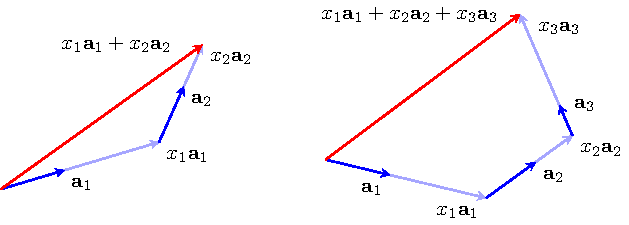
\includegraphics[scale=1.5]{lincombs.pdf}
\caption{Picturing linear combinations}
\end{figure}

\begin{exdef}\label{exdef:trivial_lc}
  The zero vector can be expressed as a	linear comination of any sequence of vectors $\bas$:
  \[ \bzero = 0\ba_1+ \cdots + 0\ba_n.  \]
  The expression on the right hand side is called the \emph{trivial linear combination} of $\bas$.
\end{exdef}

\begin{exdef}\label{exdef:standard_basis}
  Let $\bi_j\in\RR^m$ be the $j$-th column of the identity matrix $I\in\RR^{m\times m}$:
  \[
    \bi_j := \mat{0\\\vdots\\0\\1\\0\\\vdots\\0} \leftarrow \text{$j$-th row}.
  \]
  It's called the \emph{$j$-th standard basis vector of $\RR^m$}.

  Any vector $\bb\in\RR^m$ can be expressed as a linear combination of these:
\[
  \begin{array}{rcrcrcccr}
    \mat{b_1\\b_2\\\vdots\\b_m} &=&
\mat{b_1\\0\\\vdots\\0} 
&+& \mat{0\\b_2\\\vdots\\0}
&+& \cdots
&+& \mat{0\\0\\\vdots\\b_m} \\
&=& b_1\mat{1\\0\\\vdots\\0} 
&+& b_2\mat{0\\1\\\vdots\\0}
&+& \cdots
&+& b_m\mat{0\\0\\\vdots\\1} \\
&=& b_1\bi_1 &+& b_2\bi_2 &+&  \cdots  &+& b_m\bi_m
  \end{array}
\]
\end{exdef}

Here's a trivial, yet crucial, observation: By the definition of matrix multiplication,
\begin{equation}\label{eq:lc_matvec}
  x_1\ba_1+\cdots + x_n\ba_n = A\bx. 
\end{equation}
Remember this principle:
\begin{center}
  \textbf{\textit{Linear combinations are just matrix-vector products.}}
\end{center}

We apply it right away:
\begin{theorem}\label{th:col_space_is_set_of_lcs}
  The column space $C(A)$ is the set of all linear combinations of the column vectors $\bas$ of $A$:
  \[
    C(A) = \{x_1\ba_1+\cdots+x_n\ba_n : x_1,\ldots,x_n\in\RR\}.
  \]
\end{theorem}
\begin{proof}
  \begin{align*}
    C(A) &= \{A\bx : \bx\in \RR^n\}& \text{(by definition of $C(A)$)}\\
         &= \{x_1\ba_1 + \cdots + x_n\ba_n : x_1,\ldots,x_n\in \RR\} &\text{(by~\eqref{eq:lc_matvec})}.&\qedhere
  \end{align*}
\end{proof}

\section{Span}

\begin{definitions}\label{df:span}
  The \emph{span} of the vectors $\bas$, written $\spn{\bas}$, is the set of their linear combinations:
  \[ 
    \spn{\bas} := \{x_1\ba_1+\cdots + x_n\ba_n
    : x_1,\ldots,x_n\in\RR\}.
  \]
\end{definitions}

\begin{example}
  Let $\bi_1,\ldots,\bi_m$ be the standard basis of $\RR^m$, as in Example-Definition~\ref{exdef:standard_basis}. As every vector $\bb\in\RR^m$ can be expressed as a linear comnination of $\bi_1,\ldots,\bi_m$, we have
  \[
    \spn{\bi_1,\ldots,\bi_m} = \RR^m.
  \]
\end{example}

\begin{example}
  By Key fact~\ref{kf:lc_matvec} and Definition~\ref{df:col_space}, we have:
  \begin{equation}\label{eq:col_space_is_span}
    C(A) =\spn{\bas},
  \end{equation}
  where
  \[
    A=\mat{\ba_1&\ldots&\ba_n}.
  \]
\end{example}

\begin{theorem}\label{th:span_is_subspace}
  Let $\bas\in\RR^m$. Then $\spn{\bas}$ is a subspace of $\RR^m$.
\end{theorem}
\begin{proof}
  By~\eqref{eq:col_space_is_span},
  \[
     \spn{\bas}=C\left(\mat{\ba_1&\cdots&\ba_n}\right).
  \]
  Therefore, by Theorem~\ref{th:col_space_is_subspace}, $\spn{\bas}$ is a subspace of $\RR^m$.
\end{proof}

\begin{example}
  Let
  \[
    \ba_1 = \mat{1\\0\\2},\quad 
    \ba_2=\mat{-1\\-1\\0},\quad 
    \ba_3=\mat{1\\-1\\4},\quad
    \bb_1=\mat{1\\2\\3},\quad
    \bb_2=\mat{8\\3\\10}.
  \]
  \begin{enumerate}
    \item I claim that $\bb_1\notin \spn{\ba_1,\ba_2}$.

  \medskip
  It suffices to show (why?) that $\bb_1\notin C(A)$, where
  where
  \[
    A:=\mat{\ba_1&\ba_2}=\mat{1&-1\\0&-1\\2&0}.
  \]
  It is easily verified that $A\bx=\bb_1$ has no solution, so $\bb_1\notin C(A)$.


\item
  We have $\bb_2\in C(A)$ because $A\bx=\bb_2$ is soluble:

  \[
    \bx=\mat{5\\-3}
  \]
  is the unique solution.
  This solution $\bx$ to $A\bx=\bb_2$ is precisely the information we need to write $\bb_1$ as a linear comination of $\ba_1,\ba_2$:
  \[
  \mat{8\\3\\10} = \mat{1&-1\\0&-1\\2&0}\mat{5\\-3} =
  5\mat{1\\0\\2} - 3\mat{-1\\-1\\0}.
\]
By the uniqueness of the solution $\bx$, the above is the only way to write $\bb_2$ as a linear combination of $\ba_1$ and $\ba_2$.
\end{enumerate}
\end{example}








\begin{comment}
\section{Reduced row echelon form}


\begin{definition}\label{df:rref}
  A matrix $R$ is in \emph{reduced row echelon form} if:
  \begin{enumerate}
    \item All zero rows of $R$ are at the bottom.
    \item Every nonzero row has a leading one.
    \item A	leading one is the right of those in the rows above it.
    \item A leading one is the only nonzero entry in its column.
  \end{enumerate}
\end{definition}

\begin{definition}\label{df:row_equiv}
  Let $A, B\in \RR^{m\times n}$.
  We say that \emph{$A$ and $B$ are row equivalent} or that \emph{$A$ is row equivalent to $B$} if there is an \emph{invertible} matrix $\gamma\in\RR^{m\times m}$ such that $\gamma A=B$.
\end{definition}

\begin{remarks}\hfill \begin{enumerate}
  \item Since $\gamma A=B$ if and only if
	$\gamma^{-1} B=A$, the notion of row equivalence is symmetric in $A$ and $B$: $A$ is row equivalent to $B$ if and only if $B$ is row equivalent to $A$.

  \item $A$ and $B$ are row equivalent if and only if $A$ can
	be transformed into $B$ via a sequence of elementary row operations.
	The theory of elementary matrices connects this formulation of row
	equivalence with that of Definition~\ref{df:row_equiv}.
	\end{enumerate}
\end{remarks}

\begin{theorem}\label{th:rref_existence_uniqueness}
  A matrix $A$ is row equivalent to a unique matrix in reduced row echelon form.
\end{theorem}

\section{Uniqueness of reduced row echelon form} (Under construction; do not read!)

\begin{lemma}\label{L:spanofcolstotheleft} Let $A=\begin{pmatrix}\ba_1&\ba_2&\cdots\ba_n\end{pmatrix}$ be an $m\times n$ matrix reduced row echelon form with pivot columns $j_1<j_2<\ldots<j_r$. The following are equivalent:
\begin{enumerate}
\item $\ba_j$ is a pivot column of $A$.
\item $\ba_j\notin \Span\{\ba_{j_i} : j_i<j\}$.
\item $\ba_j\notin \Span\{\ba_k : k<j\}$.
\end{enumerate}
\end{lemma}
\begin{proof}
Let $A_j=\begin{pmatrix}\ba_1&\ba_2&\cdots&\ba_j\end{pmatrix}$.
Then $A_j$ is in reduced row echelon form as $A$ is (reference an exercise?) and $\{\ba_{j_i}:j_i<j\}$ is a basis for $C(A_j)$ by Theorem~\ref{T:spanofpivotcols}.
In particular, if $1\leq p\leq r$ then $\{\ba_{j_i} : 1\leq i\leq p\}$ is a basis of $C(A_{j_p})$. Since bases are linearly independent,
\[
\ba_{j_p}\notin\Span\{\ba_{j_i}: 1\leq i<p\},
\]
proving that (1) implies (2).

Conversely, suppose $\ba_j$ is not a pivot column of $A$.
Now the column space of $A_j$ is spanned by its pivot columns, namely, the $\ba_{j_i}$ with $j_i<j$, so $\ba_j\in\Span\{\ba_{j_i}:j_i<j\}$. This proves that (2) implies (1).

To see that (2) and (3) are equivalent, observe that $\Span\{\ba_k : k<j\}$ is by definition, the column space of $A_j$ while $\Span\{\ba_{j_i} : j_i<j\}$ is the span of the pivot columns of $A_j$.
But these spans are equal by Theorem~\ref{T:spanofpivotcols}.
\end{proof}

\begin{exercise}
Let $A$ be an $m\times n$ matrix in row echelon form whose leading $1$s lie in positions $(i,j_i)$, $1\leq i\leq r$. Suppose $j_i<j<j_{i+1}$. Prove that
$a_{pj}=0$ for $i< p\leq m$.
\end{exercise}


\begin{theorem}
Let $A$ and $B$ be row equivalent matrices in reduced row echelon form. Then $A=B$.
\end{theorem}

\begin{proof}
Suppose not. Then there is a pair of $m\times n$ matrices $(A,B)$ witnessing the failure of the theorem such that $n$ minimal among all such witnesses. In other words:
\begin{enumerate}
\item[(i)] $A$ and $B$ are distinct, row equivalent matrices in reduced row echelon form.
\item[(ii)] If $A'$ and $B'$ is another such pair then $A$ has fewer columns than $A'$. 
\end{enumerate}

Since $A$ and $B$ are row equivalent and in reduced row echelon form, so are $A_{n-1}$ and $B_{n-1}$. (Why?)
By the minimality of $n$, the theorem holds for $A_{n-1}$ and $B_{n-1}$. Therefore, $A_{n-1}=B_{n-1}$. Thus, to prove the theorem, it suffices to show that $\ba_n=\bb_n$.

Suppose, first, that $\ba_n$ is a pivot column of $A$.
Then $\ba_n\notin C(A_{n-1})$ by Lemma~\ref{L:spanofcolstotheleft}.
Since $A$ and $B$ are row equivalent, $\ba_n\in C(A_{n-1})$ if and only if $\bb_n\in C(B_{n-1})$.
(Row equivalence preserves linear relations between columns.)
Therefore, $\bb_n\notin C(B_{n-1})$ and, by Lemma~\ref{L:spanofcolstotheleft} again, $\bb_n$ is a pivot column of $B$.
Let $r=\rank A_{n-1}=\rank B_{n-1}$.
Then $\ba_n$ and $\bb_n$ must both equal $\be_{r+1}$ because $A$ and $B$ are in reduced row echelon form.
Thus, $\ba_n=\bb_n$.

Now suppose that $\ba_n$ is not a pivot column of $A$. Then $\ba_n\in C(A_{n-1})$ by Lemma~\ref{L:spanofcolstotheleft}, so there is a vector $\bx\in \RR^{n-1}$ such that
$\ba_n=A_{n-1}\bx$. Since $A$ and $B$ are row equivalent, $\bb_n=B_{n-1}\bx$. But $A_{n-1}=B_{n-1}$, so it follows once again that $\ba_n=\bb_n$.
\end{proof}
\end{comment}


\end{document}

